\begin{frame}
\frametitle{\textbf{Stage 2:} Prototype EDM storage ring (PTR)}

\vspace{-0.3cm}
\begin{small}
	\begin{block}{\small \textbf{Build demonstrator for charged-particle EDM}}
			\begin{itemize}
				\item Project prepared by \raisebox{-0.2\height}{
\includegraphics[height=0.4cm]{CPEDM-logo.png}} collaboration (CERN + JEDI + srEDM).
				\item  Physics Beyond Collider process (CERN) \& ESPP Update.
			\end{itemize}
	\end{block}
\end{small}

\vspace{-0.25cm}
\begin{columns}
	\column{0.675\textwidth}
\begin{block}{\small \textbf{100 m circumference}}
	\begin{small}
	\begin{itemize}
		\item $p$ at \SI{30}{MeV} all-electric CW-CCW beams operation
		\item $p$ at \SI{45}{MeV}  frozen spin including additional vertical magnetic fields
	\end{itemize}
	\end{small}
\end{block}

\column{0.25\textwidth}
    \centering
	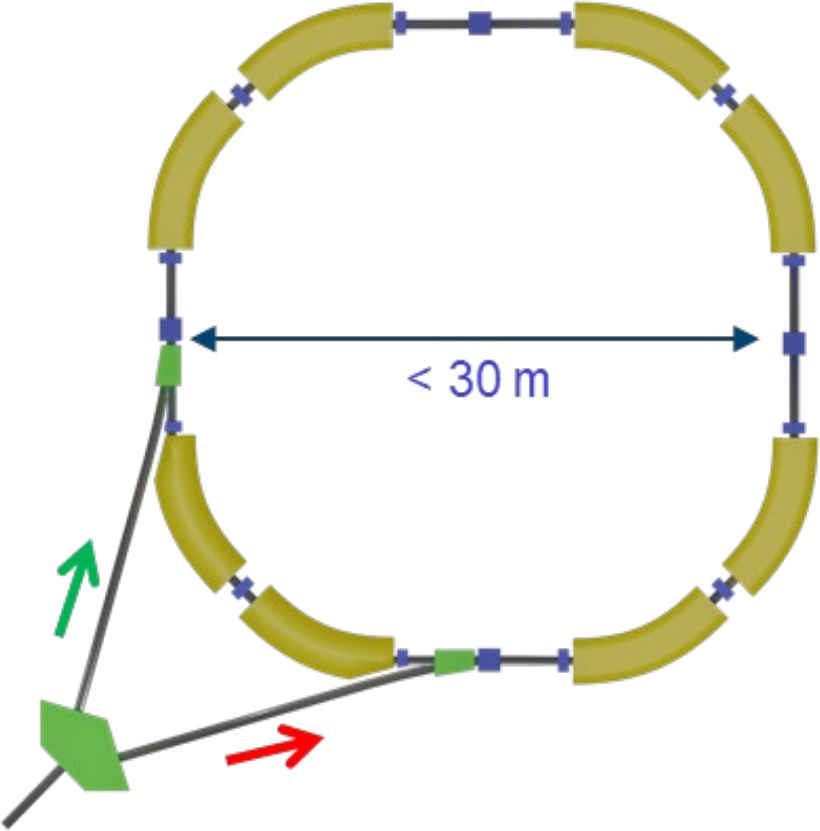
\includegraphics[width=0.55\textwidth]{PSR-topview.png}
\end{columns}

\vspace{-0.1cm}
\begin{block}{\small \textbf{Challenges -- open issues}}
	\begin{small}
	    \begin{multicols}{2}
			\begin{itemize}
				\item All electric \& $E$/$B$ combined bends
				\item Storage time
				\item CW-CCW operation with orbit difference to pm
				\item Spin-coherence time
				\item Polarimetry
				\item Magnetic moment effects (shielding) 
				\item Stochastic cooling
			\end{itemize}
		\end{multicols}
	\end{small}
\end{block}		

\vspace{-0.25cm}
\begin{alertblock}{\small \textbf{Primary purpose of PTR}}
\begin{small}
		\begin{itemize}
		\item \textbf{Study open issues and perform first direct proton EDM measurement}.
	\end{itemize}
\end{small}
\end{alertblock}
\end{frame}
%------------------------------------------------
